\section{PineAPPL at work: generation and validation of interpolation grids}
\label{sec:results}

In this section we demonstrate the capabilities of \textsc{PineAPPL} by
computing fast interpolation grids, accurate to NLO QCD and NLO QCD+EW,
for a representative set of processes in which EW corrections are expected 
to be sizeable. In order to consider some realistic kinematics for these
processes, we resort to measurements commonly devised for inclusion in PDF
fits. Our aim is twofold. First, we want to validate the results
obtained with \textsc{PineAPPL}; second, we want to assess the
impact of the EW corrections for usual experimental setups. We describe, first,
the processes and measurements that we consider, then the computational
settings that we adopt, and finally the results that we obtain.

\subsection{Processes and measurements}
\label{subsec:processes_and_measurements}

We focus on the following three processes: DY lepton-pair production, top-quark
pair production, and Z-boson (lepton-pair) production with non-zero transverse
momentum at the LHC. For each of these processes, we consider the measurements
described below.

\paragraph{DY lepton pair production.}
We select the distribution, single-differential in the invariant mass of the
lepton pair, $M_{\ell \bar\ell}$, measured by the ATLAS experiment at a centre-of
mass energy of 7~TeV in the high-mass region
($M_{\ell\bar\ell}>116$~GeV)~\cite{Aad:2013iua}.
We also select the distribution, double-differential in the rapidity and in
the invariant mass of the lepton pair, $y_{\ell\bar\ell}$ and $M_{\ell\bar\ell}$,
measured by the CMS experiment at a centre-of-mass energy of
7~TeV~\cite{Chatrchyan:2013tia}.
These measurements are currently included as standard in the
NNPDF3.1~\cite{Ball:2017nwa} and MMHT2014~\cite{Harland-Lang:2014zoa} PDF sets,
although with appropriate kinematic cuts that remove the bins at the largest
values of invariant mass, where EW corrections become sizeable.

\paragraph{Top-quark pair production.}
We select the distributions, single-differential in either the transverse
momentum of the top quark, $p_T^t$, or the invariant mass of the top-quark
pair, $m_{t\bar t}$, measured by the ATLAS and CMS experiments at a centre-of-mass
energy of 8~TeV~\cite{Aad:2015mbv,Khachatryan:2015oqa}. These measurements have
been extensively studied in the context of PDF fits in
Refs.~\cite{Czakon:2016olj,Bailey:2019yze,Amoroso:2020lgh,Kadir:2020yml}, and
included by default in the CT18~\cite{Hou:2019efy} analysis.
Because EW corrections are significantly smaller for distributions differential
in the rapidity of either the top quark or the top-quark
pair~\cite{Czakon:2017wor}, these distributions were preferred for inclusion
in the NNPDF3.1 analysis~\cite{Ball:2017nwa}.

\paragraph{$Z$-boson production with non-zero transverse momentum.}
We select the distribution, single-differential in the transverse momentum of
the $Z$ boson, $p_T^Z$, measured by the CMS experiment at a centre-of-mass
energy of 13~TeV~\cite{Sirunyan:2019bzr}. So far, this measurement has not been
included in any PDF determination. Because it has sub-percent uncertainties,
EW corrections are expected to be essential in order to achieve a good
description of it, and to constrain accurately the PDFs. Analogous measurements,
from the ATLAS~\cite{Aad:2015auj} and CMS~\cite{Khachatryan:2015oaa}
experiments at a centre-of-mass energy of 8~TeV were partly included (upon the
selection of an appropriate kinematic cut that excluded bins with large EW
corrections) in the NNDPF3.1 PDF set~\cite{Ball:2017nwa} and in variants of
the CT18 PDF set~\cite{Hou:2019efy}.

\subsection{Computational settings}
\label{subsec:computational_settings}

We generate each process by means of the Universal FeynRules Output
(UFO)~\cite{Degrande:2011ua} model {\tt loop\_qcd\_qed\_sm\_Gmu},
included as standard in {\sc MG5\_aMC}. It contains the UV and $R_2$
counterterms relevant to NLO QCD and EW corrections, the latter in the
$\overline{G}_\mu$ scheme. The model features five massless quark flavours,
sets the CKM matrix equal to the identity, and is compatible with the usage of
the complex mass (CM) scheme for all massive particles, see
Ref.~\cite{Frederix:2018nkq} for details. We use this scheme
for all processes that do not involve stable top quarks in the final state.
The photon is always considered as part of the proton in the initial state and
of any hadronic jet produced in the final state: PI effects and EW corrections
are therefore treated on the same footing. We use a PDF set that contains a
consistently defined photon PDF, namely
{\tt NNPDF31\_nlo\_as\_0118\_luxqed}~\cite{Bertone:2017bme}. We evaluate the PDF
uncertainty associated to the theoretical predictions a posteriori, that is,
we convolve the fast interpolation grid generated with {\sc PineAPPL} with
each member in the PDF set, and we compute the associated standard deviation.

The central values of the renormalisation and factorisation scales, $\mu_R$ and
$\mu_F$, are chosen, for each process, as follows. In the case of DY lepton pair
production, we use the fixed scale $\mu_R=\mu_F=M_Z$, where $M_Z$ is the mass
of the $Z$-boson, for the ATLAS measurement, and the scale
$\mu_R=\mu_F=M_{\ell\bar\ell}$, where $M_{\ell\bar\ell}$ is the central value of each
invariant mass bin, for the CMS measurement.
In the case of top-quark pair production, we use the dynamic scales
$\mu_R=\mu_F=\sqrt{m_t^2+(p_T^t)^2}{\Big /}2$ for the distribution differential
in the transverse momentum of the top quark, and $\mu_R=\mu_F=H_T/4$ for the
distribution differential in the invariant mass of the top-quark pair, where
$H_T=\sqrt{m_t^2+(p_T^t)^2}+\sqrt{m_t^2+(p_T^{\bar{t}})}$, with $m_t$,
$p_T^t$ and $p_T^{\bar t}$ the mass of the top quark and the transverse momenta
of the top and antitop quarks, respectively. These choices were demonstrated
to maximise the convergence of the perturbative expansion~\cite{Czakon:2016dgf}.
In the case of $Z$-boson production with non-zero transverse momentum, we use
$\mu_R=\mu_F=M_Z$. In order to estimate the missing higher-order uncertainty,
we allow the events to be reweighted in the Monte Carlo generation upon scale
variations. As is customary, the factorisation and renormalisation scales
are varied down to a factor $1/2$ and up to a factor $2$, and an envelope
from the seven-point scale variations is constructed.

The values of the relevant physical parameters are chosen as
\begin{equation}
%\begin{aligned}
M_\mathrm{W} = \SI{80}{\giga\electronvolt} \text{,} \quad 
M_\mathrm{Z} = \SI{91.176}{\giga\electronvolt} \text{,} \quad 
m_\mathrm{t} = \SI{172.5}{\giga\electronvolt} \text{,} \quad
\Gamma_\mathrm{W} = \SI{2.50}{\giga\electronvolt} \text{,} \quad
\Gamma_\mathrm{Z} = \SI{2.09}{\giga\electronvolt} \text{,} 
\label{eq:parameters}
%\end{aligned}
\end{equation}
where $M_W$, $M_Z$ and $m_t$ are the values of the $W$-boson, $Z$-boson and
top quark masses, respectively, and $\Gamma_W$ and $\Gamma_Z$ are the width of
the $W$-boson and of the $Z$-boson, respectively. The value of the strong
coupling is chosen consistently with the PDF set, $\alpha_s(M_Z)=0.118$.

Finally, we implement the kinematic cuts specified in the corresponding
experimental analyses. In the case of high-mass DY lepton pair
production at 7~TeV measured by ATLAS, we require $p_T^\ell>25$~GeV,
$|\eta_\ell|<2.5$ and 116~GeV$<M_{\ell\bar\ell}<$ 1500~GeV for the transverse
momentum and the rapidity of each lepton and for the invariant mass of the
lepton pair, respectively. In the case of the DY lepton-pair production at
7~TeV measured by CMS, we require $p_T^{\ell_1}>14$~GeV, $p_T^{\ell_2}>9$~GeV,
$|\eta_\ell|<2.4$, $|\eta_{\ell\bar\ell}|<2.4$ and 20~GeV$<M_{\ell\bar\ell}<$ 1500~GeV
for the transverse momentum and the rapidity of each lepton, and for the
rapidity and the invariant mass of the lepton pair. In the case of $Z$-boson
production with non-zero transverse momentum at 13~TeV measured by CMS, we
require $p_T^\ell>25$~GeV, $|\eta_\ell|<2.4$,
$M_Z$-15~GeV$<M_{\ell\bar\ell}<M_Z$+20~GeV,
$|\eta_{\ell\bar\ell}|<2.4$ and 20~GeV$<p_T^{\ell\bar\ell}<1500$~GeV for the
transverse momentum and rapidity of each lepton, and for the invariant mass,
rapidity and transverse momentum of the lepton pair.

\subsection{Numerical results}
\label{subsec:numerical_results}

For each of the measurements discussed in
Sect.~\ref{subsec:processes_and_measurements}, we compute the expectation
value of the corresponding observable for each kinematic bin in two different
ways: directly, by means of {\sc MG5\_aMC}, and a posteriori, by convolving the
fast interpolation grid produced by {\sc PineAPPL} with the PDF set specified
in Sect.~\ref{subsec:computational_settings}. In the following, we will refer
to the the first result as the {\sc MC} result, and to the second as the
{\sc PineAPPL} result. We repeat the computation for theories accurate to NLO
QCD and to NLO QCD+EW, respectively. In each case, we determine the PDF
uncertainty (coming from the PDF ensemble), the scale uncertainty (coming from
variations of the factorisation and renormalisation scales), and the Monte
Carlo uncertainty (coming from the finite number of events generated). In this
last respect, we consider by default high-statistics computations, whereby we
require a relative Monte Carlo precision of a fraction of permille. While
this choice does not affect the validation of the {\sc PineAPPL} result against
the {\sc MC} result, it ensures that the statistical uncertainty of the
computation remains negligible in comparison to the PDF and scale uncertainties,
as we will explicitly demonstrate. This is a desirable feature to correctly
interpret the size of the theoretical corrections.

Our goal is indeed twofold. On the one hand, we aim to validate the
interpolation grids generated with {\sc PineAPPL}: to this purpose we shall
verify that the MC and the {\sc PineAPPL} results are identical up to numerical
inaccuracies due to the grid interpolation. This equivalence must hold for any
choice of renormalisation and factorisation scale. On the other hand, we aim to
study the size of the EW corrections, in particular with respect to the
kinematics of each process, and to three kinds of uncertainties: the PDF
uncertainty, the scale variation uncertainty, and the uncertainty of the
experimental data.

We present these comparisons in
Figs.~\ref{fig:atlaszhighmass49fb}-\ref{fig:cmsZ13TeV} for each of the processes
and data sets outlined in Sect.~\ref{subsec:processes_and_measurements}.
The format of the plots is the same across all figures. The first panel
displays the relative difference (in permille) between the {\sc PineAPPL} and
the {\sc MC} results for the central, upper and lower scale choices, for
theories accurate to both NLO QCD and NLO QCD+EW. The following three panels
present the theoretical predictions, accurate to either NLO QCD or NLO QCD+EW,
always normalised to the former: the second displays the PDF uncertainty, the
third the scale uncertainty and the fourth the Monte Carlo statistical
uncertainty. The relative uncertainty of the experimental data points is also
shown for comparison. We shall now discuss the results for each
process and data set in turn.

\paragraph{DY lepton pair production.}




\paragraph{Top-quark pair production.}


\paragraph{$Z$-boson production with non-zero transverse momentum.}


\begin{figure}
    \centering
    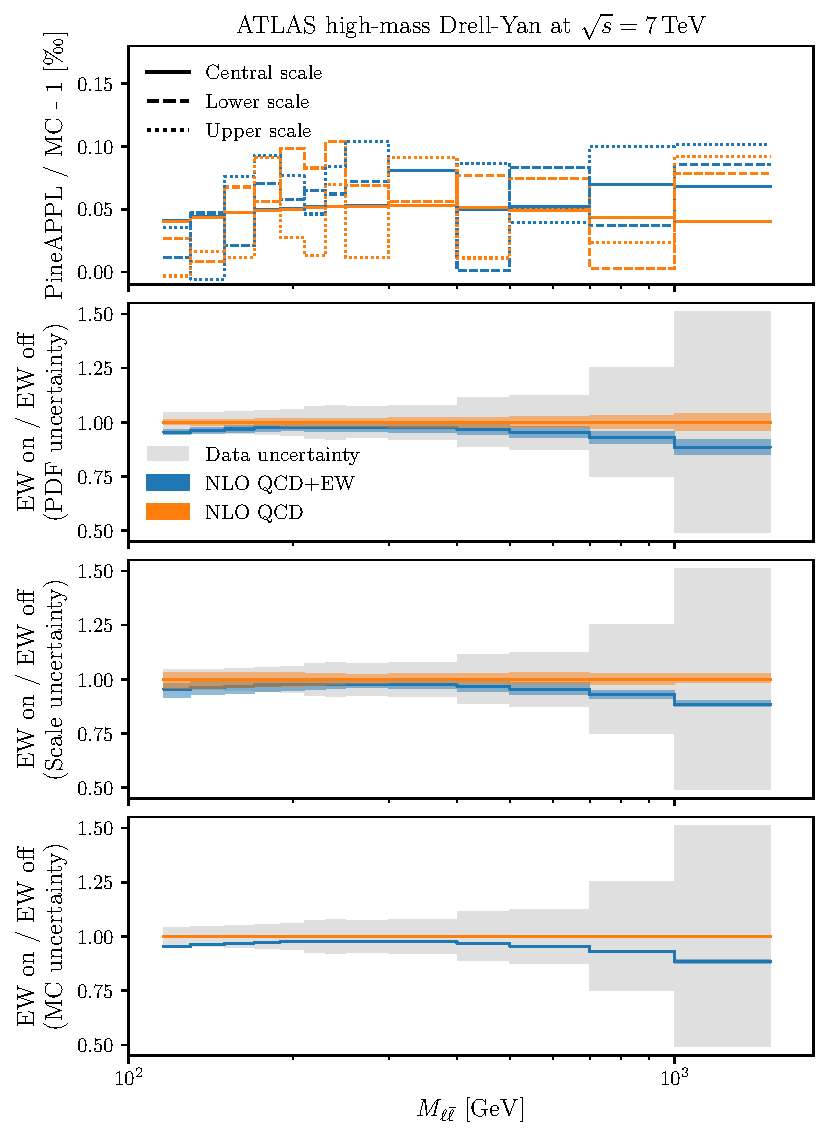
\includegraphics[width=0.5\textwidth]{figures/pineappl_ATLASZHIGHMASS49FB}
    \caption{PineAPPL comparison for ATLAS high-mass Drell--Yan at $\sqrt{s}=7$ TeV.}
    \label{fig:atlaszhighmass49fb}
\end{figure}

\begin{figure}
    \centering
    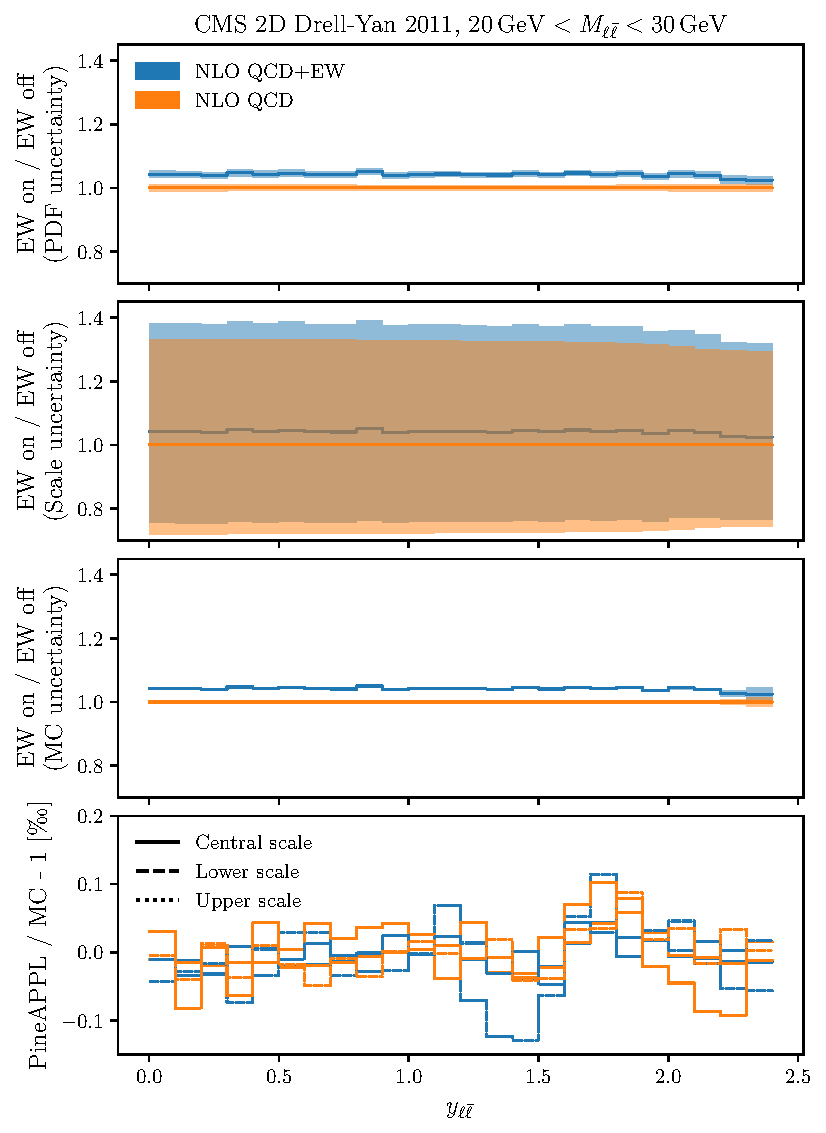
\includegraphics[width=0.5\textwidth]{figures/pineappl_CMSDY2D11_bin1}%
    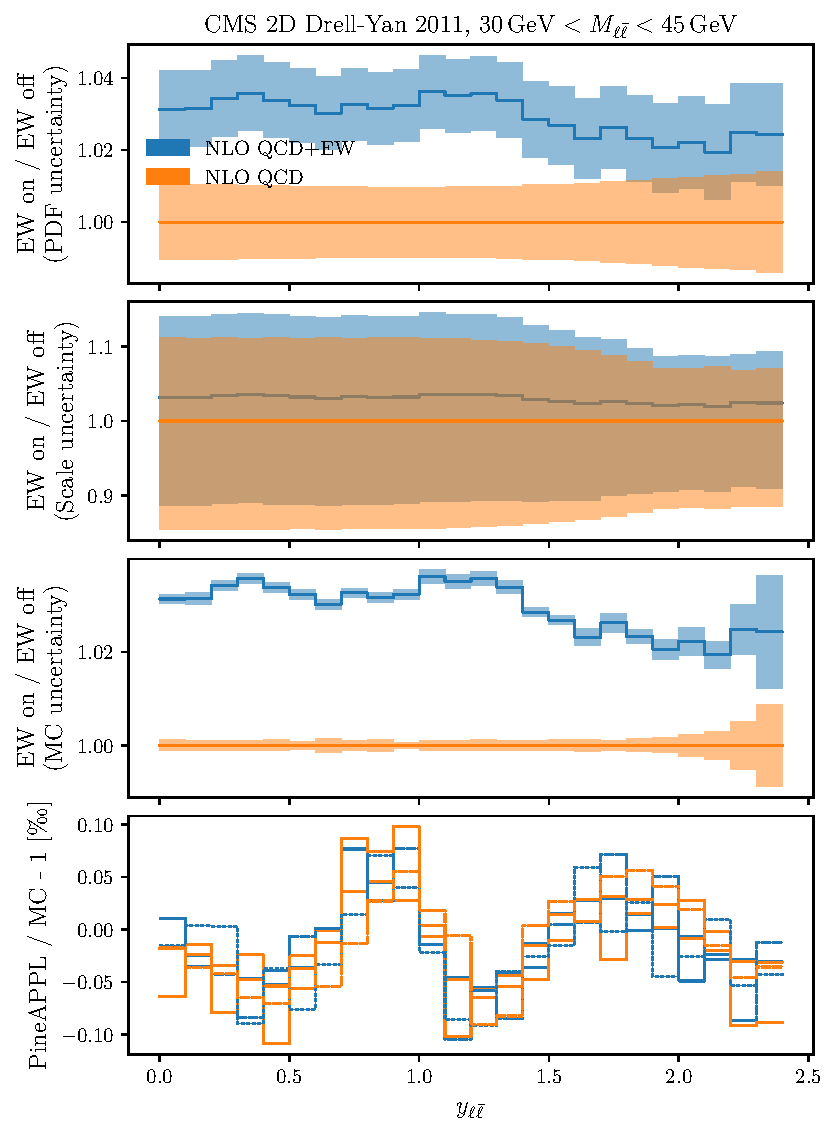
\includegraphics[width=0.5\textwidth]{figures/pineappl_CMSDY2D11_bin2}
    \caption{PineAPPL comparison for CMS 2D Drell--Yan.}
    \label{fig:cmsdy2d11_bins12}
\end{figure}

\begin{figure}
    \centering
    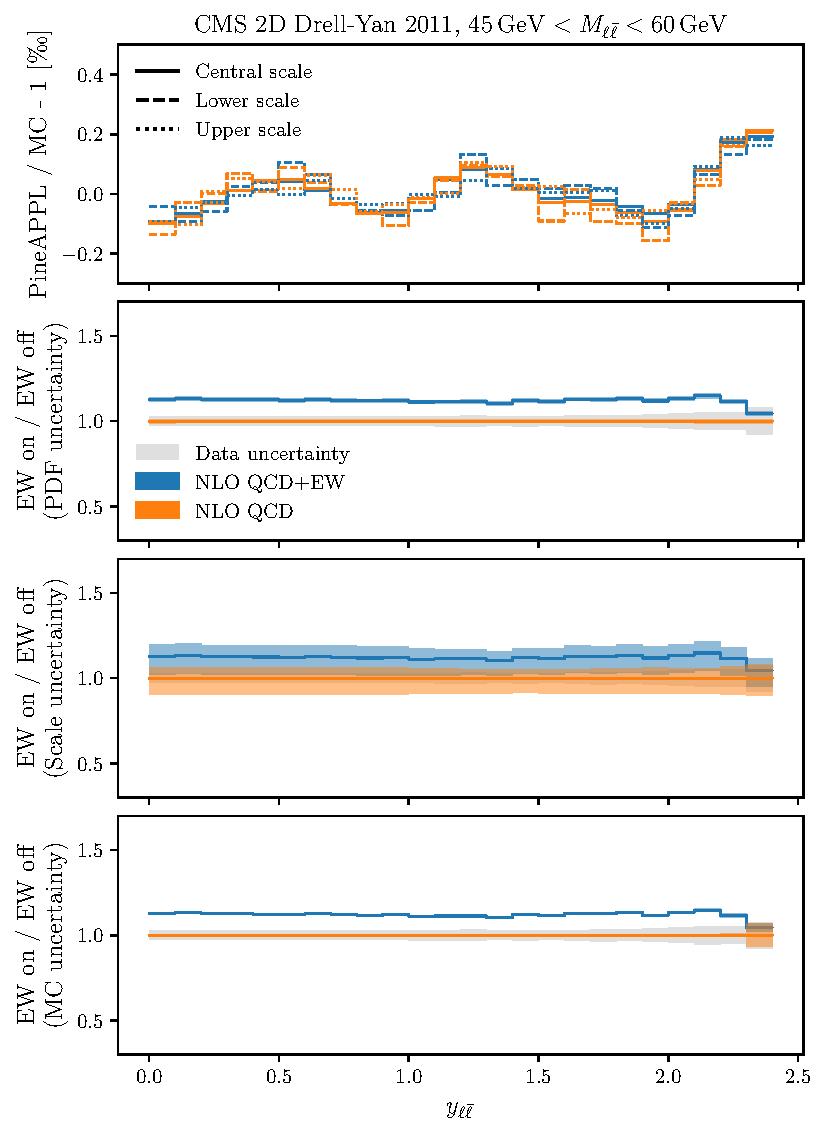
\includegraphics[width=0.5\textwidth]{figures/pineappl_CMSDY2D11_bin3}%
    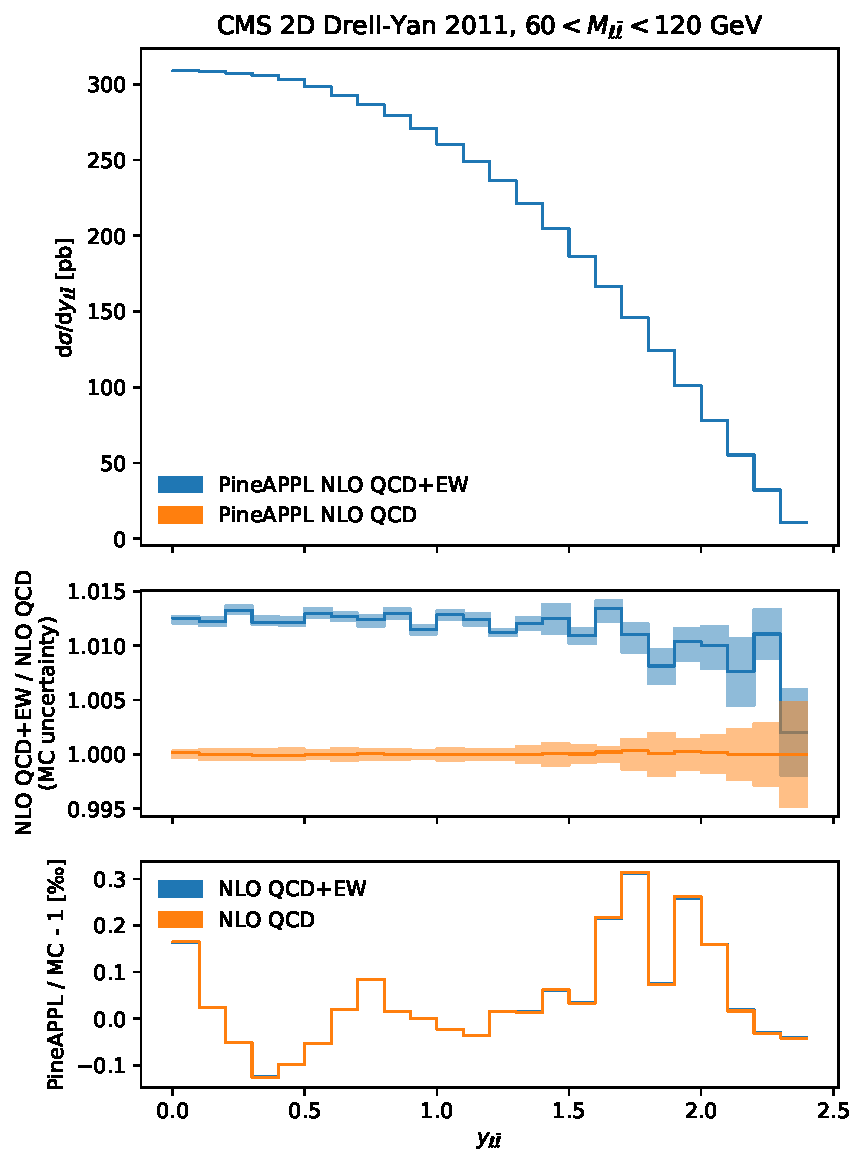
\includegraphics[width=0.5\textwidth]{figures/pineappl_CMSDY2D11_bin4}
    \caption{PineAPPL comparison for CMS 2D Drell--Yan.}
    \label{fig:cmsdy2d11_bins34}
\end{figure}


\begin{figure}
    \centering
    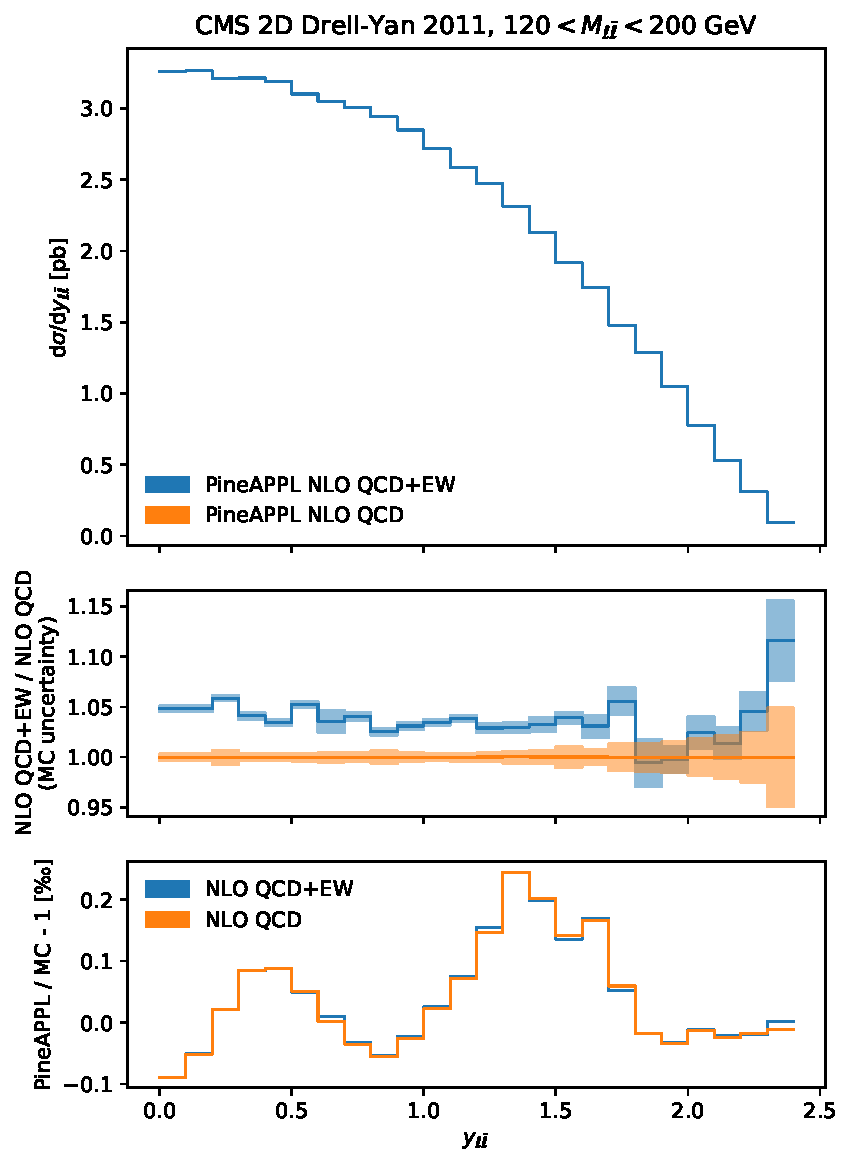
\includegraphics[width=0.5\textwidth]{figures/pineappl_CMSDY2D11_bin5}%
    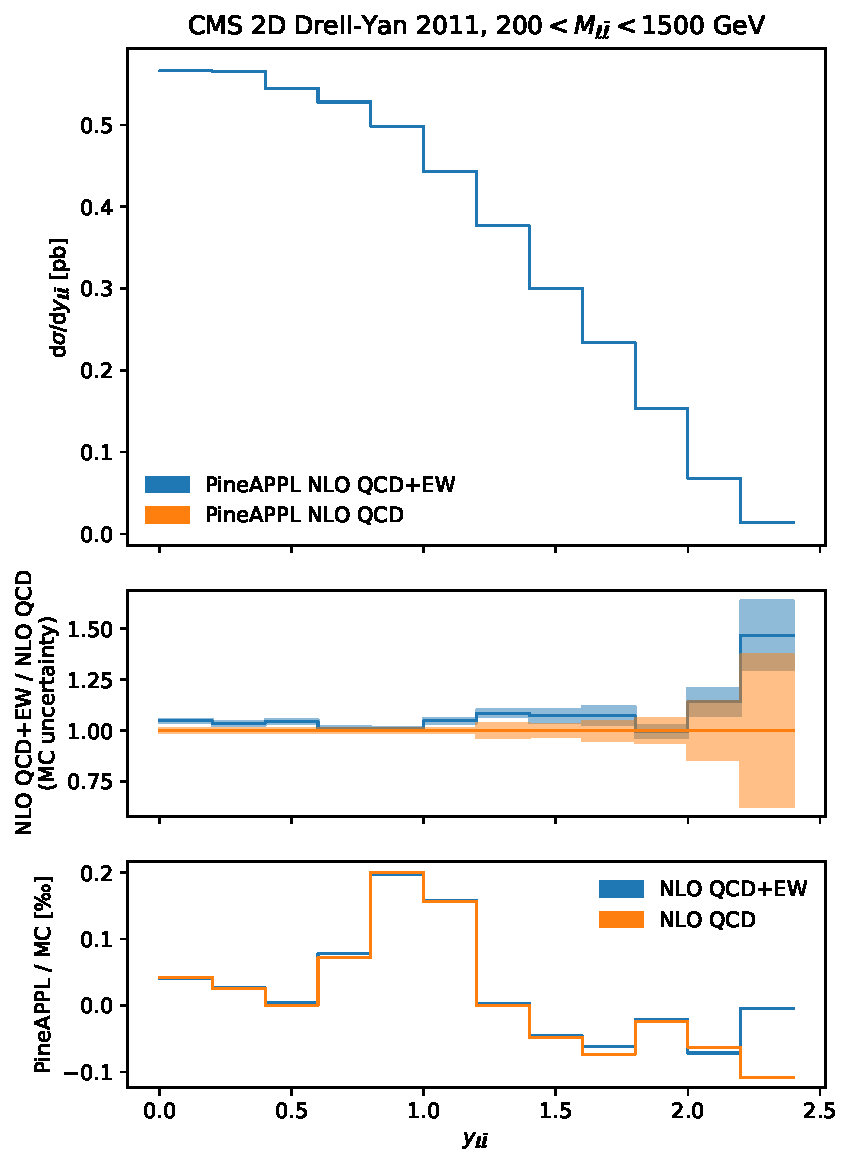
\includegraphics[width=0.5\textwidth]{figures/pineappl_CMSDY2D11_bin6}
    \caption{PineAPPL comparison for CMS 2D Drell--Yan.}
    \label{fig:cmsdy2d11_bins56}
\end{figure}


\begin{figure}
    \centering
    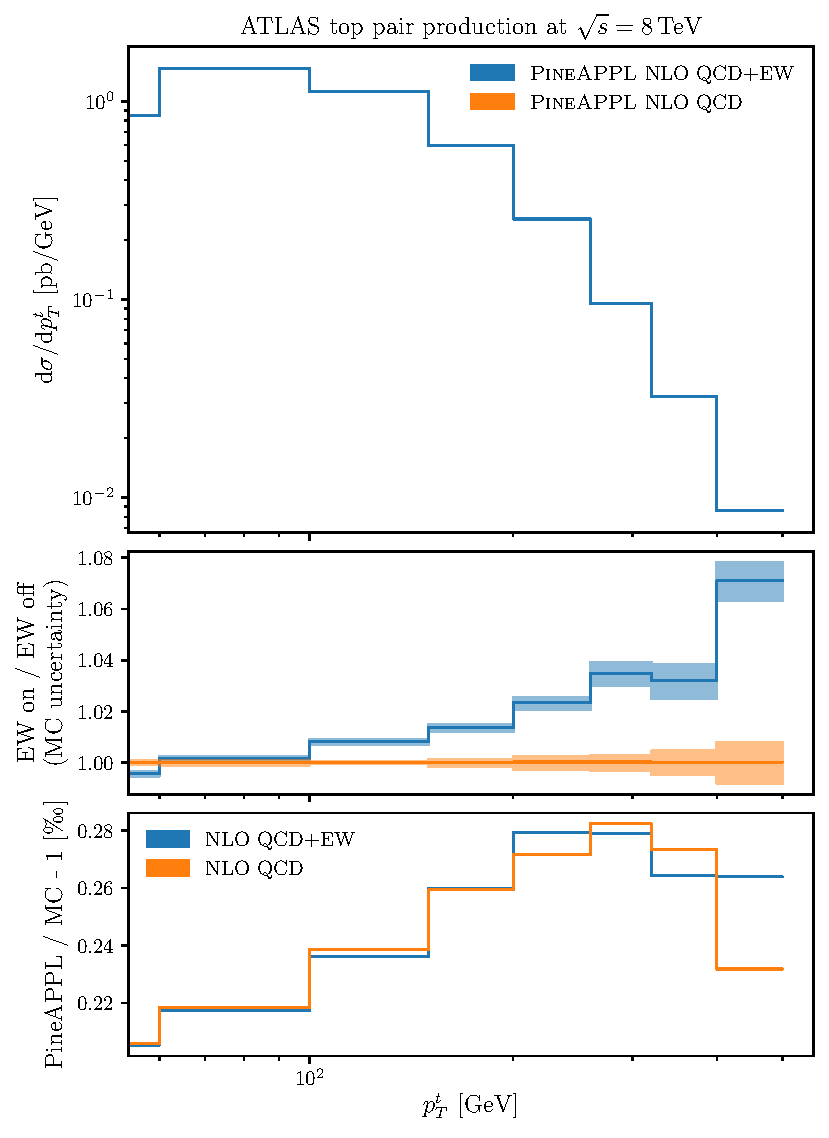
\includegraphics[width=0.5\textwidth]{figures/pineappl_ATLAS_TTB_DIFF_8TEV_LJ_TPT}%
    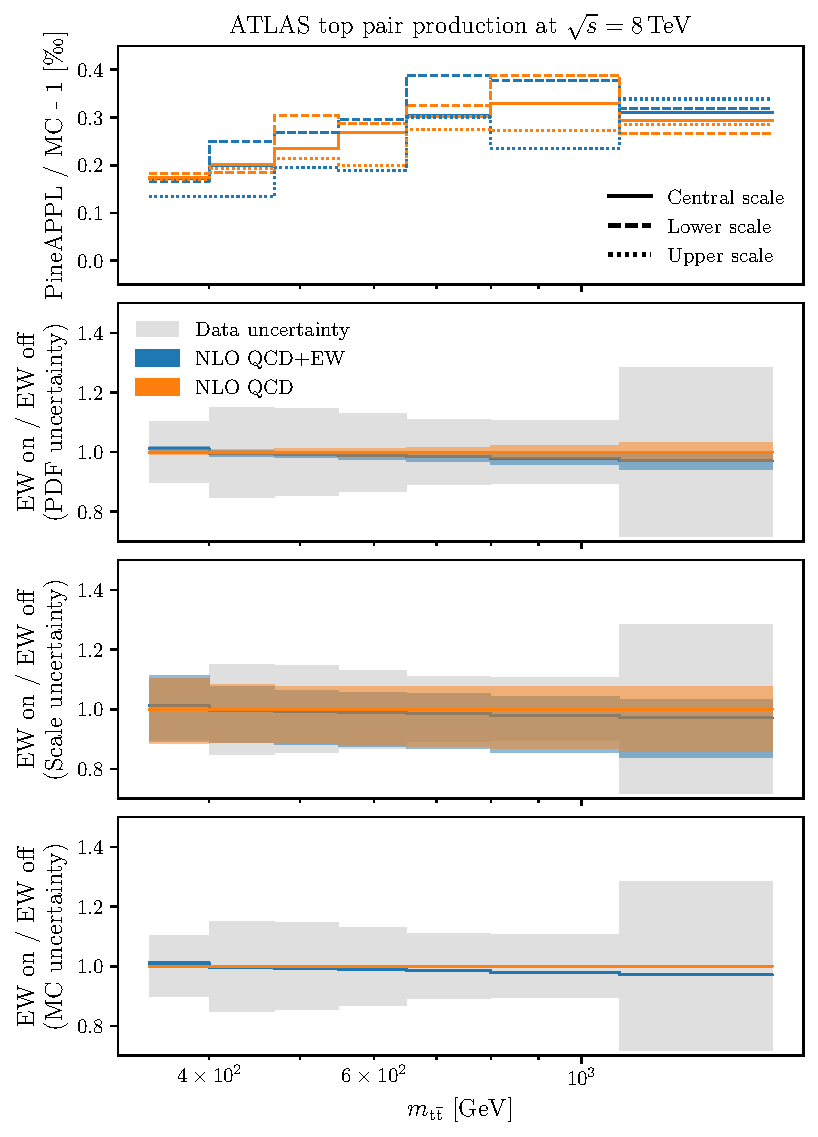
\includegraphics[width=0.5\textwidth]{figures/pineappl_ATLAS_TTB_DIFF_8TEV_LJ_TTM}
    \caption{PineAPPL comparison for ATLAS top pair.}
    \label{fig:atlastop}
\end{figure}

\begin{figure}
    \centering
    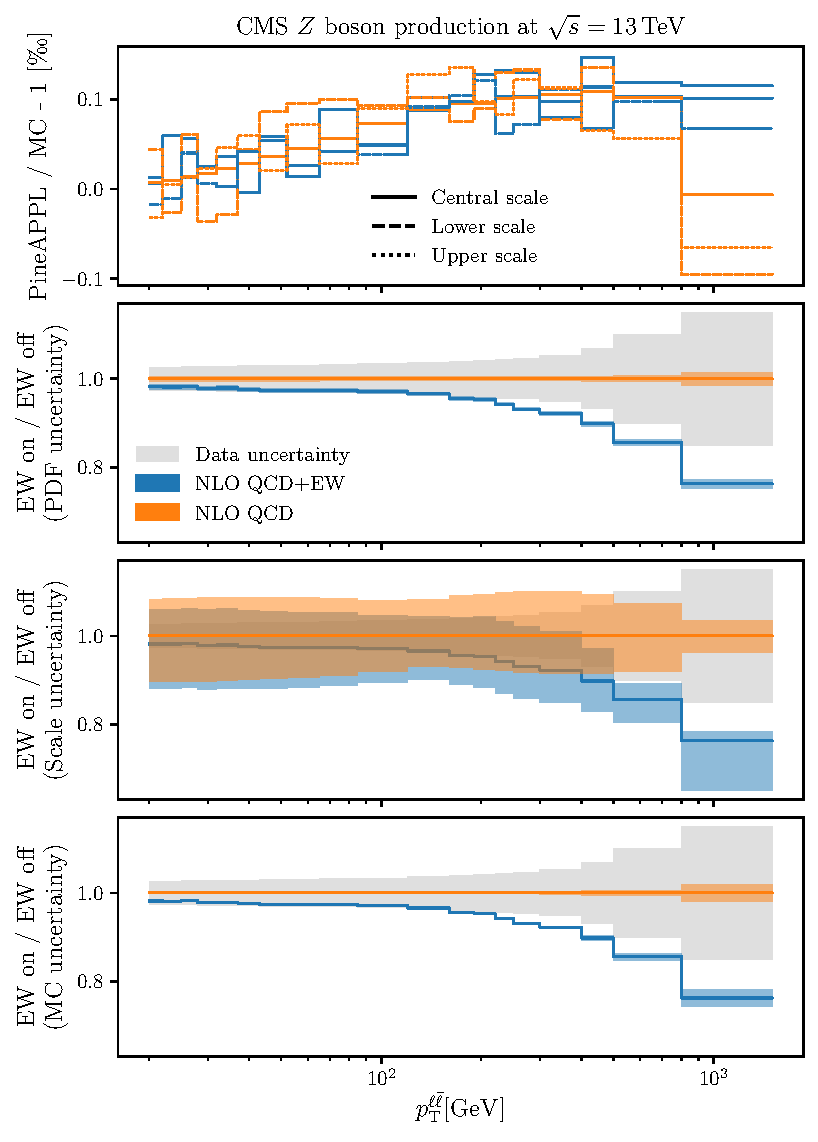
\includegraphics[width=0.5\textwidth]{figures/pineappl_CMS_Z_13_TEV}
    \caption{PineAPPL comparison for CMS $Z$ $p_T$ distribution.}
    \label{fig:cmsZ13TeV}
\end{figure}

\noindent

TODO for each process:
\begin{itemize}
\item size of the photon-initiated contributions,
\item largest partonic channel,
\item most important $x$ region,
\item PDF uncertainty,
\end{itemize}


